\section{$L^1$函数空间}\label{L1_space}
%\subsection{从空间视角看积分}
在学习数学分析/高等数学/微积分时, 我们花了很大工夫练习计算各种积分. 我依然清晰地记着被三角函数, 有理函数, 部分分式所支配的恐惧. 
\begin{figure}[h]
    \centering
    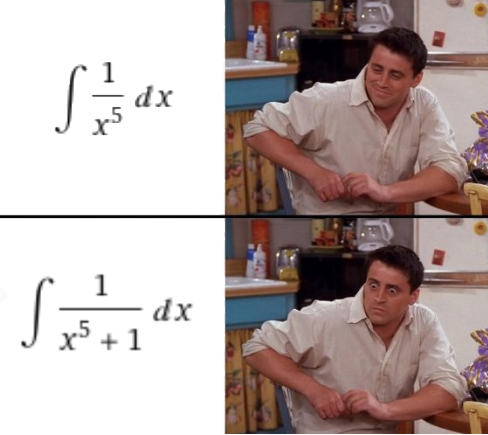
\includegraphics[scale=0.4]{image/integrate_meme.png}
    %\caption{Caption}
\end{figure}
在实分析I这里, 我们终于不(怎么)要计算啦! 掌握了勒贝格积分的定义与基本性质之后, 我们将从``空间"的视角俯瞰勒贝格可积函数构成的集合. 
什么是``空间"? 我不给出精确的定义\footnote{这个名词本身就很笼统}, 
只给出一些具体语境, 相信大家会有自己的理解.
\begin{enumerate}
    \item 称集合$V$为向量\textbf{空间}若$V$上定义了两种运算: 加法与数乘, 且它们满足众所周知的8条性质. 
    \item 称集合$X$为度量\textbf{空间}(metric space)若$X$配备了一个度量$d$. 记作$(X, d)$.
    \item 称集合$X$为赋范\textbf{空间}(normed space)若$X$配备了一个范数$\norm{\cdot}$.
    \item 称集合$X$为拓扑\textbf{空间}(topological space)若$X$配备了一个拓扑$\calT$. 记作$(X, \calT)$.
\end{enumerate}
\begin{exercise}
    再想出一个``空间"的例子.
\end{exercise}

函数列的收敛问题在分析学的历史上也算是一大热点. 
在数学分析中我们遇到过两种收敛性:
\begin{enumerate}
    \item 逐点收敛, 即$f_n(x) \to f(x)$对每个$x$都成立. 对给定的$x$, $\{f_n(x):n \in \N\}$就是个数列, 并没有什么新内容.
    \item 一致收敛, 即$\lim_{n \to \infty}f_n(x)=f(x)$对$x$一致成立, 这个要比逐点收敛复杂得多.
\end{enumerate}
逐点收敛实质上是依$\R$中的绝对值度量收敛: 一列函数$f_n$在每个点的值越来越``接近"$f$在每个对应点的值, 一致收敛实质上是依连续函数空间上的上确界范数收敛, 该范数用以衡量两个连续函数间的``距离".
在研究极限与积分运算交换次序时, 我们隐约感觉到可以用积分来衡量两个函数之间的距离. 单调收敛定理的结论为
$$\int f_n(x)dx \to \int f(x)dx \quad (n \to \infty),$$
移项得
$$\left|\int f_n(x)-f(x) dx \right| \to 0 \quad (n \to \infty).$$
该式的一个充分条件为
$$\int |f_n(x)-f(x)| dx \to 0 \quad (n \to \infty).$$
不知为什么, 这个式子看着要更顺眼一点. 将其作为衡量函数距离的尺子, 我们定义距离函数
$$d(f,g) = \int |f(x)-g(x)|dx. $$
这样
$(L^1(\R^d), d)$便成为一度量空间, 一般直接写为$L^1(\R^d)$, 或$L^1$. 
如果说度量衡量了两个函数的距离, 那么范数衡量的就是一个函数和原点(向量空间中的$0$元)的距离. 度量很自然地引导出范数:
$$\norm{f-g} = d(f, g), \quad \norm{f} = \int |f(x)|dx. $$

为了熟悉一下绝对值之外的度量/范数, 请完成该练习:
\begin{exercise}
    写出$\{f_n:n \in \N\}$依$L^1(\R^d)$的度量为一个Cauchy列的定义. 
\end{exercise}

在正课中我们学习了$L^1$空间的两大重要性质:
\begin{enumerate}
    \item 完备性: 若$\{f_n:n \in \N\}$是$L^1$中的Cauchy列, 则$f_n$在$L^1$中收敛至一个$L^1$函数$f$. 
    \item $L^1$连续性:
    $$\int |f(x+h)-f(x)|dx \to 0 \quad (h \to 0), $$
    用新型记号来写就是\footnote{有的书会定义成$\tau_h(x)=x-h$, 请以实际教材为准.}
    $$\norm{f \circ \tau_h - f}_{L^1} \to 0 \quad (h \to 0),$$
    其中$\tau_h$为平移映射, $\tau_h: \R^d \to \R^d$, $\tau_h(x) = x+h$. \\
    若定义$$F(h)=\int |f(x+h)-f(x)|dx,$$
    则有$F(h) \to 0~(h \to 0)$. 
\end{enumerate}


我们的老朋友, Riemann可积函数构成的度量空间(配备$L^1$度量)
$\calR$就没有这么好的性质. 
下面的反例说明$\calR$不完备.

\begin{example}\footnote{Fourier Analysis: An Introduction, Stein, exercise 3.5}
    令
    $$f(\theta) = \begin{cases}
        0, & \theta = 0 \\
        \log(1/\theta), & 0 < \theta \leq 2\pi,
    \end{cases}$$
    并定义$\calR$中的函数列$\{f_n: n \in \N\}$为
    $$f_n(\theta) = \begin{cases}
        0,         & 0 \leq \theta \leq 1/n \\
        f(\theta), & 1/n < \theta \leq 2\pi.
    \end{cases}$$
    证明$\{f_n: n \in \N\}$是$\calR$中的Cauchy列, 但$f \notin \calR$. 
\end{example}

% \subsection{Fourier变换初见}
% Stein Fourier Analysis Intro Chap 5 motivation
\begin{example}[~(黎曼-勒贝格引理)]
    对$L^1(\R)$中的函数$f$, 其Fourier变换为
    $\hat{f}(\xi) = \intR f(x)\FourierBase{x\xi}dx$.
    证明当$|\xi| \to \infty$时, $\hat{f}(\xi) \to 0$.
\end{example}
\begin{proof}

    由积分的平移不变性, 将$x$平移$\xi'$后不改变积分值. 于是对所有$\xi' \in \R$, 都有 
    $$\hat{f}(\xi) = \intR f(x)e^{-2\pi ix\xi}dx 
    = \intR f(x-\xi')e^{-2\pi i(x-\xi')\xi}dx.$$
    现取$\xi' = \frac{1}{2}\frac{\xi}{|\xi|^2}$, 有
    \begin{align*}
    \hat{f}(\xi) &= \intR f(x-\xi')\FourierBase{(x\xi - 1/2)}dx \\
    &= \intR f(x-\xi')\FourierBase{x\xi}e^{i\pi}dx \\
    &= -\intR f(x-\xi')\FourierBase{x\xi}dx, 
    \end{align*}
    这样我们把$\hat{f}(\xi)$写成了两种形式, 各取其半, 得 
    $$\hat{f}(\xi) = \frac{1}{2} \intR[f(x)-f(x-\xi')]\FourierBase{x\xi}dx.$$
    
    令$|\xi| \to \infty$, 则$\xi' = \frac{\xi}{2|\xi|^2} \to 0$,
    由积分的$L^1$连续性得
    $$|\hat{f}(\xi)| \leq \frac{1}{2}
     \intR|f(x)-f(x-\xi')|dx\to 0 \quad (\xi \to \infty).$$ \qed 
\end{proof}


\section{最有用的Fubini-Tonelli定理}
如果要评选出实变函数中最常用的两个定理, 我会毫不犹豫地选出“控制收敛定理”和“Fubini定理”. 
Fubini定理的核心是将重积分转化成累次积分, 而交换积分次序则是非常自然的推论. 
在应用中, Tonelli定理与Fubini定理常常成对出现. 我们往往要通过交换积分次序来降低计算难度: 按照第一种次序可能根本算不出来, 按照第二种次序可能就很快算出来了. 而只有算出来了我们才知道这个函数可不可积, 所以Tonelli定理保证了我们在不知道函数可积性的情况下也能进行换序! 
\begin{theorem}[Tonelli]
    设$f(x,y)$是定义在$\R^{d_1} \times \R^{d_2}$上的非负可测函数. 对几乎处处的$y \in \R^{d_2}$, 有
    \begin{enumerate}
    \item $f^y$在$\R^{d_1}$上可测, 
    \item 函数$y \mapsto \int_{\R^{d_1}} f^{y}(x)dx$在$\R^{d_2}$上可测,
    \item 重积分可化为累次积分:
    $$\intRd f(x,y)dxdy = \Lint{\R^{d_2}} \Brace{\Lint{\R^{d_1}}f(x,y)dx}dy.$$
    该等号在扩充实数系上也成立, 即: 若右边的累次积分等于$\infty$, 则左边的重积分也等于$\infty$ (也即$f$不可积). 
    \end{enumerate}
\end{theorem}
\begin{theorem}[Fubini]
    设$f(x,y)$在$\R^{d_1} \times \R^{d_2}$上可积. 那么对几乎处处的$y \in \R^{d_2}$, 有:
    \begin{enumerate}
    \item $f^y$在$\R^{d_1}$上可积,
    \item 函数$y \mapsto \int_{\R^{d_1}} f^{y}(x)dx$在$\R^{d_2}$上可积,
    \item 重积分可化为累次积分:
    $$\intRd f(x,y)dxdy = \Lint{\R^{d_2}} \Brace{\Lint{\R^{d_1}}f(x,y)dx}dy.$$
    \end{enumerate}
\end{theorem}
由于$x$和$y$是对等的, 所以我们很自然地推出积分次序可以交换. 如果不嫌麻烦, 不妨把定理再抄一遍:
\begin{theorem}[Fubini定理再抄一遍]
    设$f(x,y)$在$\R^{d_1} \times \R^{d_2}$上可积. 那么对几乎处处的$x \in \R^{d_1}$, 有:
    \begin{enumerate}
    \item $f_x$在$\R^{d_2}$上可积,
    \item 函数$x \mapsto \int_{\R^{d_2}} f_{x}(y)dy$在$\R^{d_1}$上可积,
    \item 重积分可化为累次积分:
    $$\intRd f(x,y)dxdy = \Lint{\R^{d_1}} \Brace{\Lint{\R^{d_2}}f(x,y)dy}dx.$$
    \end{enumerate}
\end{theorem}
这样, 以$\intRd f(x,y) dxdy$作为桥梁, 我们得到等式
$$\Lint{\R^{d_2}} \Brace{\Lint{\R^{d_1}}f(x,y)dx}dy
  =\Lint{\R^{d_1}} \Brace{\Lint{\R^{d_2}}f(x,y)dy}dx.$$
\begin{remark}
    假如要算一个函数$f(x,y)$的积分, 一般先用Tonelli定理计算$|f|$的积分(满足定理条件: 非负可测).
    把重积分转化成累次积分, 选择一个方便计算的积分次序. 
    如果算出来一个有限数, 就说明$f$可积, 再调用Fubini定理累次计算$f$的积分即可.
\end{remark}

\subsection{纯换序的计算}
接下来, 我们继续介绍Fourier变换的知识, 让大家熟悉Fubini定理的应用(顺便复习积分变量的伸缩变换). 首先来看一个无处不在(物理, 概率论, 统计学...)的函数: Gaussian.
\footnote{Gauss的形容词形式, 一般可用于形容某事物具有正态分布的特点, 也可以当作名词, 这里指形如$e^{-a|x|^2}$的函数.}
\begin{example}[~(Gaussian)]
    若$a>0$, 则
    $$I_n := \int_{\R^n}e^{-a|x|^2}dx = \Brace{\frac{\pi}{a}}^{n/2},$$
    其中$x=(x_1, \cdots, x_n) \in \R^n$, $|x|^2 = x_1^2 + \cdots x_d^2$.
\end{example}
\begin{proof}
    我们迭代地套用Tonelli定理:
    \begin{align*}
    \Lint{\R^n}e^{-a|x|^2}dx 
    &= \Lint{\R^n}e^{-a(x_1^2+\cdots+x_n^2)} dx_1 \cdots dx_n \\
    &= \Lint{\R^{n-1}}\Brace{\Lint{\R^1}e^{-a(x_1^2+\cdots+x_n^2)}dx_1 }dx_2 \cdots dx_n \\
    &= \Lint{\R^{n-1}}\Brace{\Lint{\R^1}e^{-ax_2^2-\cdots-ax_n^2}e^{-ax_1^2}dx_1} 
       dx_2 \cdots dx_n \\
    &= \Lint{\R^{n-1}}e^{-ax_2^2-\cdots-ax_n^2} \Brace{\Lint{\R^1}e^{-ax_1^2}dx_1} 
       dx_2 \cdots dx_n \\
    &= \cdots \\
    &= \Brace{\intR e^{-ax_1^2}dx_1} \cdots \Brace{\intR e^{-ax_n^2}dx_n} \\
    &= \Brace{\intR e^{-ax_1^2}dx_1}^n.
    \end{align*}
    所以只需要对$x \in \R$计算$\intR e^{-ax^2}dx$, 而我们在数学分析中见过这种积分, 参考脑海中的记忆, 由极坐标换元得
    \begin{align*}
    \Brace{\intR e^{-ax^2}dx}^2
    &= \Brace{\intR e^{-ax^2}dx}\Brace{\intR e^{-ay^2}dy} \\
    &= \iint e^{-a(x^2+y^2)} dxdy \\
    &= 2\pi \int_0^\infty e^{-ar^2}r dr \\
    &= \frac{\pi}{a}. 
    \end{align*}
    故$I_1=\sqrt{\pi/a}$. 好巧不巧, $e^{-ax^2}$还是非负的, 所以
    $$\Lint{\R^n}e^{-a|x|^2}dx = \left(\frac{\pi}{a}\right)^{n/2},$$
    这就说明$e^{-a|x|^2}$在$\R^n$上可积, 最后再由Fubini定理得$\Lint{\R^n}e^{-a|x|^2}dx = \left(\frac{\pi}{a}\right)^{n/2}$.
    \qed 
\end{proof}
% 再补一个不是非负函数的例子 (还没找好)

\begin{remark}
    大部分情况我们并不需要一板一眼地先用Tonelli定理证明可积, 再由Fubini定理得积分值. 以下的步骤足以涵盖大多数应用场景:
    \begin{enumerate}
    \item 选择合适的积分次序计算$\int |f(x,y)|dxdy$,
    \item 若算出来$\int |f(x,y)|dxdy<\infty$, 则选择合适的积分次序计算$\int f(x,y)dxdy$,
    \item 结束!
    \end{enumerate}
    如果$f$恰好是非负的, 我们只需完成第一步即可.
\end{remark}

\begin{exercise}
    假装我们已经知道$e^{-\pi x^2}$的Fourier变换是其自身:
    $$\intR e^{-\pi x^2}e^{2\pi ix \xi}dx = e^{-\pi \xi^2}, x, \xi \in \R.$$
    现设$x, \xi \in \R^d$, 计算
    \begin{enumerate}
    \item $$\intRd e^{-\pi |x|^2}\FourierBase{x \cdot \xi}dx;$$
    \item $$\intRd e^{-\pi |x|^2 / \d}\FourierBase{x \cdot \xi}dx.$$
    \end{enumerate}
\end{exercise}

在\ref{L1_space}中我们知道一个$L^1$函数的Fourier变换$\hat{f}$连续而且$\lim_{|\xi|\to \infty}\hat{f}(\xi) = 0$, 这就引出一个非常自然的问题: $\hat{f}$也可积吗? 如果$\hat{f}$也可积, 那么Fourier变换就是$L^1(\R^d)$到自身上的映射. 下面的例题否定了这个猜想. 在该例题中, 我们将会综合运用以下知识点:
\begin{itemize}
    \item 积分变量的伸缩性质
    \item Fubini定理
    \item $\Ga$函数的性质\footnote{如果忘了$\Ga$函数, 可参考任一数学分析教材或者本讲义的附录}
    
\end{itemize}
\begin{example}\footnote{Real Analysis, Stein, exercise 2.25}
    {\everymath{\displaystyle}
    证明对每个固定的$\eps > 0$, 关于$\zeta$的函数$F(\xi)=\frac{1}{(1+|\xi|^2)^\eps}$
    是某个$L^1$函数的Fourier变换. \\
    \textbf{提示}: 令$K_\delta(x)=e^{-\pi|x|^2/\delta} \delta^{-d/2}$, 考虑
    $f(x)=\int_0^\infty K_\delta(x)e^{-\pi \delta}\delta^{\eps-1} d\delta$. 
    应用Fubini定理证明$f \in L^1(\R^d)$, 且$$\hat{f}(\xi) = \int_0^\infty e^{-\pi \delta |\xi|^2} e^{-\pi \delta} \delta^{\eps-1} d\delta, $$
    然后计算这个积分(用gamma函数表达), 结果应为
    $\pi^{-\eps}\Gamma(\eps)\frac{1}{(1+|\xi|^2)^\eps}$.
    }
\end{example}
\begin{proof}
    \begin{align*}
    \intRd f(x)dx
    &= \intR \Brace{\intRd e^{-\pi |x|^2/\d}dx}e^{-\pi \d}\d^{-\frac{d}{2}+\eps-1}d\d \\
    &= \intR \Brace{\frac{\d}{\pi}\pi}^{d/2}e^{-\pi \d}\d^{-\frac{d}{2}+\eps-1}d\d \\
    &= \intR e^{-\pi \d}\d^{\eps-1}d\d \\
    &= \pi^{1-\eps}\intR e^{-\pi \d}(\pi\d)^{\eps-1}d\d \\
    &= \pi^{-\eps}\intR e^{-\pi \d}(\pi\d)^{\eps-1}d(\pi\d) \\
    &= \pi^{-\eps}\Ga(\eps) < \infty,
    \end{align*}
    hence $f \in L^1(\R^d)$. Next, 
    \begin{align*}
    \hat{f}(\xi)
    &= \intRd f(x) \FourierBase{x\cdot \xi}dx \\
    &= \intR_d \Brace{\intR e^{-\pi |x|^2/\d} e^{-\pi \d}\d^{-\frac{d}   {2}+\eps-1} d\d} \FourierBase{x\cdot \xi}dx \\
    &= \intR \Brace{\intRd e^{-\pi |x|^2/\d}
       \FourierBase{x\cdot \xi}dx}e^{-\pi \d} % another FT
       \d^{-\frac{d}{2}+\eps-1} d\d \\
    \end{align*}
    Let $g(x)=e^{-\pi|x|^2/\d},$ then $g(\d^{1/2}|x|)=e^{-\pi|x|^2}$, 
    so $g(\d^{1/2}|x|) \longrightarrow \d^{-d/2}\hat{g}(\d^{-1/2}\xi) = e^{-\pi|\xi|^2}$. From this we get $\hat{g}(\xi)=\d^{d/2}e^{-\pi \d|\xi|^2}$. 
    Continue,
    \begin{align*}
    \hat{f}(\xi)
    &= \int_0^\infty e^{-\pi \delta |\xi|^2} e^{-\pi \delta} \delta^{\eps-1} d\delta \\
    &= \intR e^{-\pi(1+|\xi|^2)\d}\d^{\eps-1}d\d \\
    &= \intR e^{-\pi(1+|\xi|^2)\d}(\pi(1+|\xi|^2)\d)^{\eps-1}
       (\pi(1+|\xi|^2))^{1-\eps} d\d \\
    &= \pi^{-\eps}(1+|\xi|^2)^{-\eps} 
       \intR e^{\pi(1+|\xi|^2)\d}(\pi(1+|\xi|^2)\d)^{\eps-1} 
       d(\pi(1+|\xi|^2)\d) \\
    &= \pi^{-\eps}\Ga(\eps)\frac{1}{(1+|\xi|^2)^\eps}
    \end{align*}
    Once $\eps$ is given, $\Ga(\eps)$ is a constant. 
    We have shown that $\pi^{-\eps}\Ga(\eps)\frac{1}{(1+|\xi|^2)^\eps}$ is the Fourier transform of $f$. \qed
\end{proof}
\begin{remark}
    If we take $\eps=1/2$ and let $d=1$ 
    then calculus tells us 
    $$ \int \frac{1}{\sqrt{1+\xi^2}}d\xi 
       = \log (\xi + \sqrt{\xi^2 + 1}) + C, $$
    hence $\intR \frac{1}{\sqrt{1+\xi^2}}d\xi$ diverges. 
\end{remark}

\subsection{积分区域的切片}
不知大家有没有发现, 刚才几个例子的积分区域\footnote{这里的区域泛指做积分的可测集, 而非有界开集}
都是$\R$或者更一般的$\R^n$, 所以我们在换序时不需要考虑积分区域的变化. 回忆一下我们在微积分/数学分析中是怎么计算二重积分的: 将积分区域写成所谓的``$x$型区域"或``$y$型区域", 再进行累次积分. 
而在Fubini定理中, 积分区域看似都是$\R^d, \R^{d_1}, \R^{d_2}$, 实则吸收于被积函数$f$中: $$\int_E f(x,y) dxdy = \intRd f(x, y) \chi_E (x,y) dxdy. $$
做累次积分就会出现
$$\int_{\R^{d_1}} f(x,y) \chi_E (x,y) dx, $$
此时被积函数就可看作$y$固定, $x$在动的切片$(f \chi_E)^y(x) = f^y(x) (\chi_E)^y(x)$. 考虑$d_1=d_2=1$的二重积分情形, $(\chi_E)^y(x)$ 与积分号 $
\intR$ 碰一碰就能产生
$$\intR f^y(x) (\chi_E)^y(x) dx = \int_{E^y} f^y(x) dx!$$
这就是我们在微积分中做的事: 找切片区域. 我们马上看一个具体的例子:
\begin{example}[~(分布函数)]
    设$f$是$\R^d$上的可测函数, 定义$f$的\textit{分布函数}$d_f: [0, \infty) \to [0, \infty]$为 
    $$d_f(\a) = m(\{x \in \R^d: |f(x)| > \a\}).$$ 
    设
    $|f|^p \in L^1, 0<p<\infty$.
    证明
    $$\|f\|_{L^p}^p := \intRd |f|^p d\mu = p \int_0^\infty \a^{p-1}d_f(\a) d\a. $$
\end{example}
\begin{proof}
    将分布函数中的测度还原成积分形式, 得
    \begin{align*}
    p \int_0^\infty \a^{p-1}d_f(\a) d\a
    &= p \int_0^\infty \a^{p-1} \int_X \chi_{\{x:|f(x)|>\a\}} dm(x) 
        d\a. 
    \end{align*}
    开始换序! 我们需要给特征函数做切片, 严格复制粘贴定义得
    $$\chi_{\{x:|f(x)|>\a\}}(x, \a) = 
    \begin{cases}
        0 & \text{若 } |f(x)| \leq \a, \\
        1 & \text{若 } |f(x)| > \a.
    \end{cases}$$
    固定住$x$, 则$\chi$的$x$-切片为
    $$\chi_{\{x:|f(x)|>\a \}}(\a) = 
    \begin{cases}
        0 & \text{若 } \a \geq |f(x)|, \\
        1 & \text{若 } \a < |f(x)|.
    \end{cases}$$
    所以, 
    \begin{align*}
    p\int_0^\infty \a^{p-1} \intRd \chi_{\{x:|f(x)|>\a\}} dm(x)d\a
    &= p\intRd \int_0^\infty \a^{p-1} \chi_{\{x:\a < |f(x)| \}}(\a) d\a dm(x) \\
    &= \intRd \int_0^{|f(x)|} pa^{p-1} d\a dm(x) \\
    &= \intRd |f(x)|^p dm(x).
    \end{align*}
    \qed
\end{proof}
\begin{remark}
    在微积分中, 积分区域一般都是矩形, 三角形等肉眼可以看出切片的集合, 但在实分析中我们遇到的大多是抽象的集合, 正如上例. 强烈建议初学者严格按照``特征函数 $+$ 在整个空间上积分"的形式进行计算. 
\end{remark}
\begin{exercise}
    设$f \in L^1(\R)$, 令$F(x) = \int_{-\infty}^x f(t)~dt$, 证明$F$连续.
\end{exercise}